\section{Evaluation} \label{sec:eval}
As has been acknowledged multiple times, memory consumption is one of the largest bottlenecks for Dinur's polynomial-method solver. From \cite{eurocrypt-2021-30841}, it is known that the procedure will store $2^{n - 2n_1}$ solutions in each round, in expectation. Workarounds for this was also introduced in that same paper, with alternatives introduced here as well. Therefore, \cref{sec:eval:mem} is dedicated to evaluating the memory consumption of the current implementation. Further, since the effectiveness of the procedure was shown, also in \cite{eurocrypt-2021-30841}, to be largest for rather large polynomial systems, \cref{sec:eval:dinur_fes} looks at how the implementation fares against an alternative procedure that has been tested and used in practice more than a few times. At last, \cref{sec:eval:large} examines how the implementation handles "larger" parameter sizes, while \cref{sec:eval:future} evaluates the work behind the implementation instead of its performance.

\subsection{Memory consumption} \label{sec:eval:mem}

For a visual comparison of the three most prominent C variants, refer to \cref{fig:mem_dinur}. The figure displays the memory consumption on these variants, in \texttt{MiB}, across the time they spent solving the system. The system can be found in the \texttt{report/metrics/memory/} folder, alongside the \texttt{.dat} files used to for plotting this figure and the \texttt{procinfo\_} files used later in this subsection.

It should be noted that the graphs in \cref{fig:mem_dinur} are all measured via the \texttt{run.py} python script, implying that some amount of memory will also be allocated for Python and SageMath related elements, like the interpreter. However, large parts of the SageMath-induced memory consumption also stems from things like storing the input system as a list of SageMath polynomials prior to calling the shared library. This would potentially be better if a frontend was developed in language more similar to C. From testing, around 200-230 \texttt{MiB} are used up until the C library is called, when run on systems like those used in \cref{fig:mem_dinur}.

\begin{figure}[t]
    \centering
    \begin{tikzpicture}   
        \begin{groupplot}[
            group style={
                group size=3 by 1,
                x descriptions at=edge bottom,
                y descriptions at=edge right,
                yticklabels at=all,
                group name=mem plots,
            },
            xlabel={Time in seconds},
            ylabel={Memory consumption (\texttt{MiB})},
            ymajorgrids=true,
            grid style=dashed,
            ymin=200,
        ]
        \nextgroupplot
            \addplot[
                color=blue,
            ] table [header=false,x expr=\coordindex/10,y index=1]{metrics/memory/mprofile_32_31.dat};
        \nextgroupplot
            \addplot[
                color=blue,
            ] table [header=false,x expr=\coordindex/10,y index=1]{metrics/memory/mprofile_128_31.dat};
        \nextgroupplot
            \addplot[
                color=blue,
            ] table [header=false,x expr=\coordindex/10,y index=1]{metrics/memory/mprofile_256_31.dat};
        \end{groupplot}
        \node[below = 1cm of mem plots c1r1.south] {(a)};
        \node[below = 1cm of mem plots c2r1.south] {(b)};
        \node[below = 1cm of mem plots c3r1.south] {(c)};
    \end{tikzpicture}
    \caption{Memory consumption for three variants of the C implementation on a system with $n = m = 31$. (a) \textit{Standard} C version; compiled to use 32-bit registers. (b) SIMD version; 128-bit AVX registers. (c) SIMD version; 256-bit AVX registers.} \label{fig:mem_dinur}
\end{figure}

\subsubsection{Standard}

Inspecting graph (a) in \cref{fig:mem_dinur}, it is quite clear that the solver spent three rounds to solve the entire system. The memory consumption gradually increases up until around around 30 seconds, at which it point it falls and not long after starts increasing again. Similar "hitches" in the increasing memory consumption can be seen at around 50-60 seconds. These increases are as expected, given that the procedure has to store large amounts of solutions at each round, comparing newly found candidates to previous ones.

The expected amount of memory for storing solutions is about $4(n_1 + 1) \cdot 2^{n - n_1}$ bits, in expectation (theoretically). Of course, this comes stems from allocating full $(n_1 + 1) \times 2^{n - n_1}$-sized tables for storing candidate solutions in each round. Storing these bits in single bytes would yield a memory consumption of 
$$
    \frac{4 \cdot 8 \cdot 2^{31 - 7}}{2^{20}} = 512
$$
\texttt{MiB} in total, for a naive implementation. In comparison, storing the solutions bit-sliced, combining the $n_1 + 1$ bits into a single byte would yield a $64$ \texttt{MiB} memory consumption. At last, storing only candidate solutions would yield
$$
    \frac{2^{31 - 2 \cdot 7} \cdot 4}{2^{20}} = 0.5
$$
\texttt{MiB} of memory, in expectation. This last calculation assumes that all $31$ bits of a solution are stored in a single $32$-bit integer. Now, remember, these calculations are purely theoretical as they do not take into account elements like memory alignment, storage of \texttt{struct}s, stack usage, and memory consumption as a whole.

Since candidate solutions are stored using an array of \texttt{poly\_t}, the memory allocated for storing solutions is rather close to 4 bytes per stored solution. In \texttt{report/metrics/memory/bench\_output} other data from the standard run can be found. From this file, the amount of stored solutions can be read, which totalled $31\,952\,544$ solutions. This means that around
$$
    \frac{31\,952\,544 \cdot 4}{2^{20}} \approx 122
$$
\texttt{MiB}s were used for storing solutions alone. This amount of storage fits quite nicely with what can be derived from \cref{fig:mem_dinur}a, but is not comparable to the $2^{31 - 2 \cdot 7}$ expected candidates. Running the standard solver on similar system sizes yields the same results. Due to time constraints, the exact condition triggering this was not discovered. Some plausible factors could elements like sampling of system polynomials, sampling of random matrices or various analytical assumptions made when proving the complexity of the algorithm. This latter case can relate to the two former ones, as the analysis in \cite{eurocrypt-2021-30841} made certain assumptions that may not be entirely met in practice (on the distribution of these samplings).

Nevertheless, from the theoretical 512 \texttt{MiB} of storage the standard implementation manages to cut down the memory consumption, based on the experimental evidence. Also note, even though bit-slicing the $(n_1 + 1) \times 2^{n - n_1}$ table theoretically yields a smaller memory consumption than the experimental one, for the same parameter sizes, this does prove a time-memory trade-off. Packing solutions sequentially can yield more cache-friendliness, especially considering that the access patterns in the table of solutions is quite linear no matter how the solutions are iterated. Another point is that a $(n_1 + 1) \times 2^{n - n_1}$ (even if bit-sliced) requires one to potentially iterate all $2^{n - n_1}$ keys, instead of only ever accessing the relevant solutions.

In \cref{fig:three_mem}, more general comparison of memory strategies is shown. The curves are shown up to $n = 32$, since the samples stem from an implementation using 32-bit integers for solutions. The \textit{full-sized} and \textit{bit-sliced} curves represent the theoretical values as a function of $n$, where $n_1 = \lceil \frac{n}{5.4} \rceil$. The third curve is fit from averages across five runs for 10 different parameter sets. Clearly, this more general picture shows the same story as the single sample from \cref{fig:mem_dinur}. Of course, the curve may be more accurate if more samples were used, or the averages computed for more systems. Therefore, \cref{fig:three_mem} should not taken as an exact science, but does hint at the aforementioned trend in the relationship between the three memory strategies. Also, the major \textit{hitches} in the blue and green curves stem directly from the value of $n_1$ changing, which would yield quite different results if the $\frac{n}{2.7d}$ were used specifically (as proposed in \cite{eurocrypt-2021-30841}).

\begin{figure}[t]
    \centering
    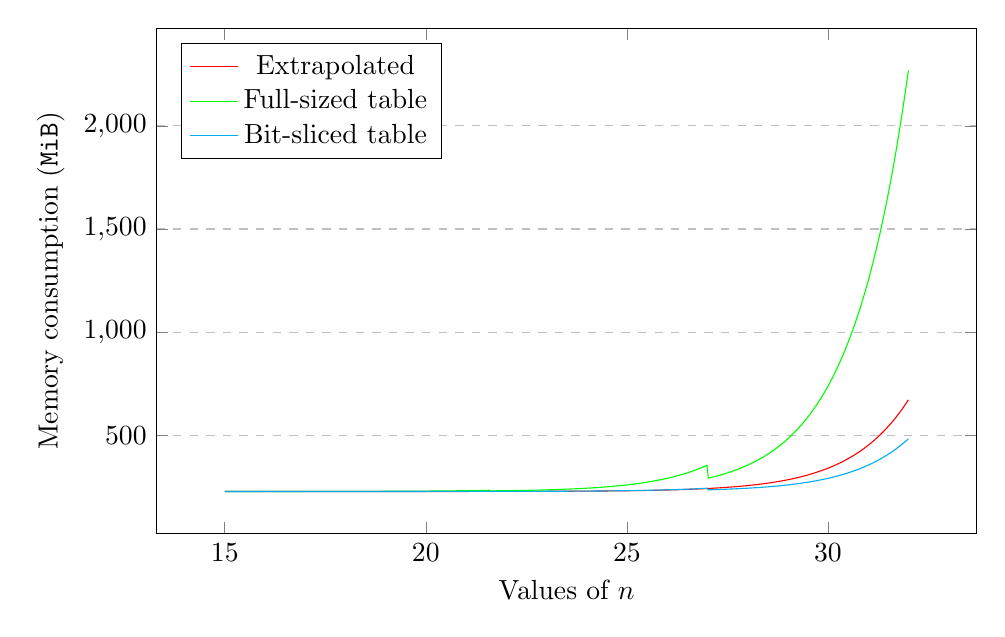
\begin{tikzpicture}
        \begin{axis}[
            xlabel=Values of $n$,
            ylabel=Memory consumption (\texttt{MiB}),
            xtick={15,20,25,30},
            height=8cm,
            width=12cm,
            ymajorgrids,
            grid style=dashed,
            legend pos=north west,
        ]
        \addplot[
            color=red,
            domain=15:32,
            samples=500,
        ]
        {(0.00013831083126693568 * 2^(0.988135062636788 * x) + 232634.0051135452)/1024};
        \addplot[
            color=green,
            domain=15:32,
            samples=500,
        ] {(4 * 8 * 2^(x - (ceil(x/5.4)))/1024 + 232634.0051135452)/1024};
        \addplot[
            color=cyan,
            domain=15:32,
            samples=500,
        ] {(4 * 2^(x - (ceil(x/5.4)))/1024 + 232634.0051135452)/1024};
        \legend{Extrapolated, Full-sized table, Bit-sliced table}
        \end{axis}
    \end{tikzpicture}
    \caption{Three strategies for storing solutions, where one curve was fit from actual memory consumption data on systems from $n = m = 20$ to $n = m = 30$. The two others are purely based on theoretical expected values. Memory data is sampled from \texttt{/proc/<pid>/status}.} \label{fig:three_mem}
\end{figure}

Now, to sum up the memory consumption of the standard implementation; the implementation acts much as expected theoretically, given how solutions are stored. Although the consumed memory is less than a by-the-books storage mechanism, the trend is still exponential in nature and therefore a great bottleneck. With \textit{compact} storage mechanism used for solutions, it uses more memory than if elements were bit-sliced. If $n > 32$, the extrapolated red curve would need to be revised on samples from an implementation using 64-bit integers, which would also drastically increase memory consumption (potentially $31$ wasted bits in each integer). The two theoretical curves would also need to be revised when $n > 37$, as the evaluations of the $U$ polynomials ($n_1 + 1$ bits) no longer fits into a byte. However, the general nature is still tend towards the trend shown in \cref{fig:three_mem}. Finally, due to the non-deterministic nature of the solver, the amount of solutions stored may differ when running the solver on one system multiple times. Expectedly, no drastic changes would occur with high frequency, but it is still a risk.

\begin{figure}[t]
    \centering
    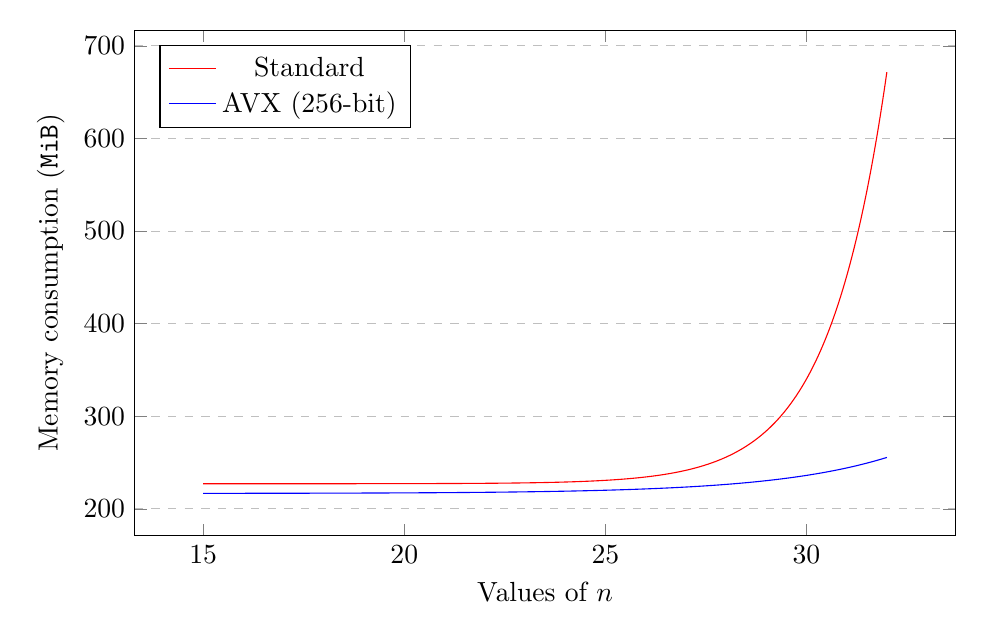
\begin{tikzpicture}
        \begin{axis}[
            xlabel=Values of $n$,
            ylabel=Memory consumption (\texttt{MiB}),
            xtick={15,20,25,30},
            height=8cm,
            width=12cm,
            ymajorgrids,
            grid style=dashed,
            legend pos=north west,
        ]
        \addplot[
            color=red,
            domain=15:32,
            samples=500,
        ]
        {(0.00013831083126693568 * 2^(0.988135062636788 * x) + 232634.0051135452)/1024};
        \addplot [
            color=blue,
            domain=15:32,
            samples=500,
        ] {(0.6300250132482776 * 2^(0.4984381599371818 * x) + 221906.00452997335)/1024};
        \legend{Standard, AVX (256-bit)}
        \end{axis}
    \end{tikzpicture}
    \caption{Memory consumption plotted as functions of $n$ for the \textit{standard} and \textit{vectorized} implementations. The \textit{standard} curve is the same as the extrapolated curve in \cref{fig:three_mem}. Memory data is sampled from \texttt{/proc/<pid>/status}.} \label{fig:avx_simd_mem}
\end{figure}

\subsubsection{SIMD}
As already explained, one of the key goals for the vectorized implementation was to better handle the memory consumption. By storing multiple systems $\Tilde{\mathcal{P}^{(i)}_k}$ (for $k = 0, \dots 4$) the solution processing and checking can be handled simultaneously inside the interpolation/evaluation procedure \texttt{fes\_recover()}. This way, no solution needs to be stored other than the one currently being processed by \texttt{fes\_recover()}, as the vectorization allows for computing multiple solutions in parallel.

The fact that solutions are not stored in large arrays should be clear from \cref{fig:mem_dinur}, as both graphs (b) and (c) does not yield the same slow increase in memory as graph (a). Mostly, the two SIMD implementations seem rather close in their memory consumption, even though ones register is double the size. With an observant eye, it can be seen that the 256-bit AVX implementation has a larger memory consumption, however, more precise profiling of the memory usage would be needed to say if it is exactly double. Of course, the memory usage as a whole is not expected to be double, as the two implementations mostly store non-vectorized elements the same. Also recall that the SageMath frontend sets a strong baseline in memory consumption before any C procedures are called. 

For a closer inspection of the memory consumption when compared to the standard implementation, observe \cref{fig:avx_simd_mem}. The two curves are sampled from different data points gathered from 5 runs of 10 different parameter sets. Now, as explained in \cref{sec:impl:opt}, the memory consumption of the vectorized implementation still acts like an exponential function in $n$, due to the relationship between $w$ and $n$. Even though both implementations store exponential amounts of memory, the vectorized implementation has a drastically slower growth, as \cref{fig:avx_simd_mem} clearly shows. This exponential growth stems from the storage of the derivative table in \texttt{fes\_recover()}, which holds $\sum_{i = 0}^{w + 1} \binom{n - n_1}{i}$ vectors.

The expected memory consumption for the derivative table alone is at most 
$$
    32 \cdot \sum_{i = 0}^{\lceil \frac{n}{5.4} \rceil + 3} \binom{n - n_1}{i}
$$
bytes as $w \leq 2 (n_1 + 1) - n_1$ when solving quadratic systems. By using \cref{fig:mem_dinur} as a reference, this would yield a total an upper-bound of $3\,918\,016$ bytes, or $\approx 4$ \texttt{MiB}. 

Typically, the storage of AVX vectors in main memory requires specifically aligned memory, as alternatively specialized instructions (with worse performance) are needed. This alignment, 32 bytes for 256-bit vectors and 16 bytes for 128-bit vectors, should be taken into consideration when comparing the theoretical $4$ \texttt{MiB} of storage to what is displayed in \cref{fig:mem_dinur}. An interesting element of graphs (b) and (c) is the sudden increase in memory consumption early on in the procedure. Since the vectorized implementations fixes $q$ variables and stores $2^q$ new system of $n - q$ variables, the memory build-up is expected quite large early on. Furthermore, the storage of derivative tables (exponentially sized) also occur soon after variables have been fixed, and so the memory increase seen in those regions of (b) and (c) is probably heavily attributed to these storage solutions. 

Comparing graphs (b) and (c) (\cref{fig:mem_dinur}) to graph (a), a strength of the vectorized implementations is how the memory consumption essentially reaches a static maximum. Once \texttt{fes\_recover\_vectorized()} as allocated derivative tables and other memory areas, no real increase happens. This solution is therefore more predictable in the consumed memory. The vectorized implementations neither risk storing many solutions, in the extreme case where the solver has to spend a lot more than four rounds to find a solution. Of course, the trade-off of the vectorized approach is still the limit of \texttt{only} storing four rounds worth of values for each fixed system, possibly not catching some candidates that would otherwise have been catched.

The general trend seen from \cref{fig:mem_dinur} and \cref{fig:avx_simd_mem} is that the vectorized implementation comparably manages to tackle the memory issues of Dinur's algorithm in a more efficient manner. As will be seen in \cref{sec:eval:dinur_fes}, taking timings into consideration does not hurt the vectorized implementation either.

\subsection{Time} \label{sec:eval:dinur_fes}
\td{CHANGE}
In this subsection, the performance of the different implementations is compared against that of a similarly optimized FES implementation for quadratic polynomials. Here "similarly optimized" means that the procedure is optimized in the same ways as that of \texttt{fes\_eval\_parity()}, the underlying FES-procedure for \texttt{fes\_recover()} and Dinur's \texttt{BRUTEFORCE()} method (see \cref{alg:uvalue}). This . This section will also do internal comparisons between the vectorized/SIMD and standard implementation of Dinur's algorithm. 

\subsubsection{Standard and vectorized versions}
With the current implementations, both vectorized and non-vectorized, the algorihms did not beat the FES implementation in \texttt{src/c/standard/fes.c} on samples of smaller systems. The implementation(s) were not tested on systems larger than $n = m = 48$, however, the vectorized version was ran on using multiprocess implementation on such a system specifically (see \cref{sec:eval:large}).

\begin{table}[t]
    \begin{center}
        \pgfplotstabletypeset[
            col sep=comma,
            columns={Compile_config,g_solve_time,g_recover_time,g_hist_time},
            every row 2 column 2/.style={{postproc cell content/.style={@cell content=-}}},
            every row 2 column 3/.style={{postproc cell content/.style={@cell content=-}}},
            every row 1 column 3/.style={{postproc cell content/.style={@cell content=-}}},
            columns/Compile_config/.style={
                column name=Compile config,
                string type,
                string replace={fes64}{FES},
            },
            columns/g_solve_time/.style={
                column name=Solve time,
                postproc cell content/.append style={
                        /pgfplots/table/@cell content/.add={}{ ms}
                },
            },
            columns/g_recover_time/.style={
                column name=Total recovery time,
                postproc cell content/.append style={
                    /pgfplots/table/@cell content/.add={}{ ms},
                },
            },            
            columns/g_hist_time/.style={
                column name=History checking,
                postproc cell content/.append style={
                    /pgfplots/table/@cell content/.add={}{ ms},
                },
            },
            every even row/.style={
                before row={
                  \rowcolor[gray]{0.9}
                }
            },
            every head row/.style={
                before row=\toprule,
                after row=\midrule
            },
            every last row/.style={
                after row=\bottomrule
            },
       ]{metrics/fes_dinur/bench_30_30.csv}
    \end{center}
    \caption{A comparison of different procedures solving a system of $n = m = 30$. The timings are averages from 10 different systems of this size.} \label{tbl:comp_perf_30}
\end{table}

Consider \cref{tbl:comp_perf_30}, which shows average timings for solving 10 different systems of $n = m = 30$ using the three algorithms of interest. In these tests, the vectorized implementation obtains approximately a 20 times speedup over the non-vectorized implementation in total solve time. In \cref{tbl:total_comp_perf} much the same picture is drawn. The speedup from the standard version to the vectorized version is not a perfect 20 times at each parameter-set, however, the general trend is that at least a 20 times speedup is seen. Again, these measurements are not a perfect science but do show a trend. 

An interesting characteristic for the timings of the standard version is that the increase in solve time seems to be \textit{slower} in some parameter-ranges. For instance, at $n = m \in \{27, 28\}$ and $n = m \in \{21,22\}$ (\cref{tbl:total_comp_perf}) the increase in time is either very slow or upright negative. Examining the behavior of the function that determines $n_1$, i.e. $n_1 = \lceil \frac{n}{5.4} \rceil$, the \textit{stepping} nature of the ceiling function shows directly in the timings. For both $n = m \in \{27, 28\}$ and $n = m \in \{21,22\}$, the \texttt{fes\_recover()} procedure (being the dominating contributor to timings) iterates through $2^{17}$ and $2^{22}$ values of the $\mathbf{y}$-bits, respectively. In other cases, the increase is essentially exponential. This would of course have looked different, had $n_1$ been computed differently.

\begin{table}[t]
    \begin{center}
        \pgfplotstabletypeset[
            col sep=comma,
            columns={standard,vectorized,fes,n},
            columns/standard/.style={
                column name=Standard,
                postproc cell content/.append style={
                    /pgfplots/table/@cell content/.add={}{ ms}
                },
            },
            columns/vectorized/.style={
                column name=Vectorized,
                postproc cell content/.append style={
                        /pgfplots/table/@cell content/.add={}{ ms}
                },
            },
            columns/fes/.style={
                column name=FES,
                postproc cell content/.append style={
                    /pgfplots/table/@cell content/.add={}{ ms},
                },
            },
            columns/n/.style={
                column name={$n,m$},
            },   
            every even row/.style={
                before row={
                  \rowcolor[gray]{0.9}
                }
            },
            every head row/.style={
                before row=\toprule,
                after row=\midrule
            },
            every last row/.style={
                after row=\bottomrule
            },
       ]{metrics/fes_dinur/bench_comp.csv}
    \end{center}
    \caption{A comparison of total solve times for different procedures solving different system sizes. The timings are averages from 10 different systems of this size.} \label{tbl:total_comp_perf}
\end{table}

By fitting exponential curves onto the data from \cref{tbl:total_comp_perf} one obtains \cref{fig:time_dinur_fes}. From these curves, the general trend from the timings of \cref{tbl:total_comp_perf} are shown more clearly. As a function of the number of variables, $n$, the solve times tend to grow a lot quicker than those of the vectorized implementation. As can be seen in \cref{tbl:comp_perf_30}, a large contributor to the overall solve time is the history-checking phase. In \cref{sec:eval:mem}, the amount of stored candidate solutions was disclosed as being a lot more than theoretically expected. Since timings for history-checking is directly correlated to how many candidate solutions are stored, a non-negligible amount of time could be saved.

\begin{figure}[t]
    \centering
    \begin{tikzpicture}
        \begin{groupplot}[
            group style={
                group size=2 by 1,
                x descriptions at=edge bottom,
                y descriptions at=edge right,
                yticklabels at=all,
                group name=time plots,
            },
            xlabel={Value of $n$},
            ylabel={Average solve time (seconds)},
            ymajorgrids=true,
            grid style=dashed,
            height=7cm,
            width=7cm,
            legend pos=north west,
        ]
        \nextgroupplot
            \addplot [
                color=red,
                domain=15:32,
                samples=500,
            ] {(0.00013821278616837966 * 2^(1.0287978391219936 * x) + 7680.478916011137)/1000};
            \addplot [
                color=blue,
                domain=15:32,
                samples=500,
            ] {(4.515335132855728e-06 * 2^(1.0492286454281707 * x) + 154.5501396250078)/1000};
            \addplot [
                color=black,
                domain=15:32,
                samples=500,
            ] {(9.743886211109144e-06 * 2^(0.9886510877075164 * x) + -6.710511139391242)/1000};
            \legend{Standard, AVX (256-bit), FES} 
        \nextgroupplot
            \addplot [
                color=blue,
                domain=15:32,
                samples=500,
            ] {(4.515335132855728e-06 * 2^(1.0492286454281707 * x) + 154.5501396250078)/1000};
            \addplot [
                color=black,
                domain=15:32,
                samples=500,
            ] {(9.743886211109144e-06 * 2^(0.9886510877075164 * x) + -6.710511139391242)/1000};
            \legend{AVX (256-bit), FES} 
        \end{groupplot}
        \node[below = 1cm of time plots c1r1.south] {(a)};
        \node[below = 1cm of time plots c2r1.south] {(b)};
    \end{tikzpicture}
    \caption{(a) A plot of the fitted curves for all three procedures. (b) A zoom-in on the curves for the vectorized implementation and basic FES implementation.} \label{fig:time_dinur_fes}
\end{figure}

Further, the largest contributor to solve times for both implementations of the algorithm is the FES-based recovery. This is expected, given that this procedure replaces the Möbius transform interpolation and evaluation, both being large contributors to the complexity of the original algorithm. With \cref{tbl:fes_comp_perf} the distribution of time spent evaluating and interpolating can be read, as well as the overall recovery-time. Of course, this recovery time also includes checking evaluations for $U_0(\hat{\mathbf{y}}) = 1$, and household tasks like memory allocation. These contributions clearly do affect the timings quite a lot, but for now the thesis will focus on total timings for evaluation and interpolation.

From the samples in \cref{tbl:fes_comp_perf}, larger parameter-sizes seem to change the balance of interpolation and evaluation. In the lower rows of the table, interpolation is the slowest part but in the upper rows the roles are reversed. It was expected that interpolation would be the slowest of the two, as this included both running \texttt{fes\_eval\_parity()} internally, as well as interpolating derivative table entries. Examining the evaluation part of \texttt{fes\_recover()}, many operations are rather simple in nature, except indexing. It turns out that the indexing operation is quite a heavy operation when computed as in \cref{lst:c:index}. This computation is also performed often, and as $n - n_1$ increases, the amount of evaluations expectedly increases. The heaviest operation of the evaluation is indexing and must for this reason also act as a large contributor to interpolation times, especially on smaller parameter-sizes. To be more clear, as n increases, more vectors in $\{0,1\}^{n - n_1}$ will have a hamming-weight greater than \texttt{deg}, triggering evaluation instead of interpolation (see \cref{alg:fes_recover}).
\td{NOT GOOD ENOUGH EXPLANATION?}
\begin{table}[t]
    \begin{center}
        \pgfplotstabletypeset[
            col sep=comma,
            columns={recovery,interpolation,evaluation,n},
            columns/recovery/.style={
                column name=Recovery,
                postproc cell content/.append style={
                    /pgfplots/table/@cell content/.add={}{ ms}
                },
            },
            columns/interpolation/.style={
                column name=Interpolation,
                postproc cell content/.append style={
                        /pgfplots/table/@cell content/.add={}{ ms}
                },
            },
            columns/evaluation/.style={
                column name=Evaluation,
                postproc cell content/.append style={
                    /pgfplots/table/@cell content/.add={}{ ms},
                },
            },
            columns/n/.style={
                column name={$n,m$},
            },   
            every even row/.style={
                before row={
                  \rowcolor[gray]{0.9}
                }
            },
            every head row/.style={
                before row=\toprule,
                after row=\midrule
            },
            every last row/.style={
                after row=\bottomrule
            },
       ]{metrics/fes_dinur/bench_recover.csv}
    \end{center}
    \caption{A comparison of FES-based recovery timings (non-vectorized), and internal timings, for different system sizes. The timings are averages from 10 different systems of this size.} \label{tbl:fes_comp_perf}
\end{table}

\subsubsection{Comparing against FES}

For the sake of comparison, both the standard and vectorized implementation was compared to a FES implementation for quadratic systems. As already explained, this implementation was optimized in pretty much the same way as \texttt{fes\_eval\_parity()} in \texttt{src/c/standard/fes.c}. A comparison of the total solve times can once more be found in \cref{tbl:total_comp_perf}. With an almost perfect doubling from $n = m = 20$ to $n = m = 30$, the FES procedure manages to outperform even the vectorized implementation of Dinur's algorithm. As is depicted by the fitted exponential curves in \cref{fig:time_dinur_fes}b, simple FES implementation manages to outperform the vectorized implementation by around a factor two, quite consistently. Comparing the standard implementation to the FES implementation, the performance speedup of FES is downright distressing for the standard implementation of Dinur's algorithm. Using the functions of \cref{fig:time_dinur_fes}a, no crossover point can be found, for which FES would be slower than Dinur's algorithm.

Many reasons may exist for these gloomy performance results when compared to FES, a few of which possibly already disclosed by earlier sections. Nonetheless, the comparison is still important as it shows the reality of these implementations. Although many time contributors (in practice) were disclosed in former sections, the analysis of \cite{eurocrypt-2021-30841} does make certain assumptions. First off, the paper focuses on cryptographically relevant parameter-ranges, which the samples from \cref{tbl:total_comp_perf} are not even near. Also, even though the complexity measure is \textit{bit operations} (and non-asymptotic), certain operations are declared negligible and thereby ignored for the total amount of bit operations. As the tests ran here are classified as smaller systems (in 2023 at least), these \textit{negligible} performance contributors may actually have had relevance for the data sampled and curves being fitted. An example of a \textit{negligible} term in the analysis of \cite{eurocrypt-2021-30841} is the interpolation of polynomials using the Möbius transform (when compared to the \texttt{BRUTEFORCE()} procedure of \cref{alg:uvalue}). In the data sampled in \cref{tbl:fes_comp_perf}, although only for the standard implementation, the interpolation of polynomials holds a significant proportion of the total recovery time. Of course, comparing the theoretical analysis to practically sampled data is not a one-to-one mapping for many reasons. One such reason being that the analysis is based on the use of the Möbius transform, and the samples are based on a FES-based recovery approach (\cref{sec:ext}).

\subsection{Solving large systems} \label{sec:eval:large}
Using the data from \cref{tbl:total_comp_perf}, and thereby curves of \cref{fig:time_dinur_fes}, to extrapolate the time it would take to solve a large system will not provide optimistic results. For a 48-variable system in 48 polynomials, the authors of \cite{ches-2010-23990} found all common zeros in 21 minutes. By extrapolating the time to solve a 48 variable system (in 48 polynomials) using the sampled data from the former sections, the result is around 1816 hours, or 75 days. This extrapolation is from the data on the vectorized implementation, i.e. the fastest of the two. Of course, it could be argued that more samples would be needed to provide more accurate predictions, however, this would likely not show competitive results (compared to established solvers like FES). 

Instead of trying to solve a system for 75 days on a single core, a 48 variable system in 48 equations was attempted solved on a multicore machine. The attempt was run on a 128 core (256 thread) x86-based machine. The vectorized implementation using 256-bit AVX registers, running in parallel on 256 threads, managed to solve such a system in about 25 hours. Recall from \cref{sec:impl:opt} that running on a multicore system, the procedure fixes $\log_2 q$ variables on $q$ core machines. This meant that $\log_2 256 = 8$ variables were fixed before handing the $2^8$ new systems to individual CPU threads. 

Now, compare the solve-time to the single-core AVX (again, 256-bit vectors) implementations by, once more, extrapolating the solve times. In a perfectly scaled world, the total solve time of the multicore run would match solving an $n = 48 - 8 = 40$ system. Extrapolating the single-core timings, a system of $n = 40$ would be solved in about 5 hours. Instead, a system of $n = 42$ would be solved in about 23 hours, according to the extrapolated data, being more comparable to the 25 hours of the multicore version on $n = m = 48$. Of course, neither the samples, nor the world, are perfect. The multicore implementation is handled by Python/SageMath and the \texttt{multiprocesing} library, meaning that the fixing of variables and bit-slicing is handled here as well. Having the overhead of Python/SageMath on fixing and bit-slicing could prove part guilty for this non-perfect scaling. 

% Turning the attention to the results of \cite{ches-2010-23990}, one may wonder if the GTX 295 (used in said paper) is comparable to a 256 thread x86 machine. In some sense, the amount of cores would make it comparable to older GPUs, however, as GPU cores are more specialized toward certain operations. The authors of \cite{ches-2010-23990} note that a GPU version of their algorithm had around a 13 times speedup when compared to one of the fastest consumer-grade CPUs available at the time. 

% Extrapolations and actual results.

\newpage